\begin{frame}[t]{Nastavenie parametrov}
\begin{itemize}
  \item<1-> Napr. v Mission Planner nájdeme všetky Eulerove uhly + výšku, polohu, rýchlosť

  \begin{onlyenv}<1>
  \begin{figure}
\centering
  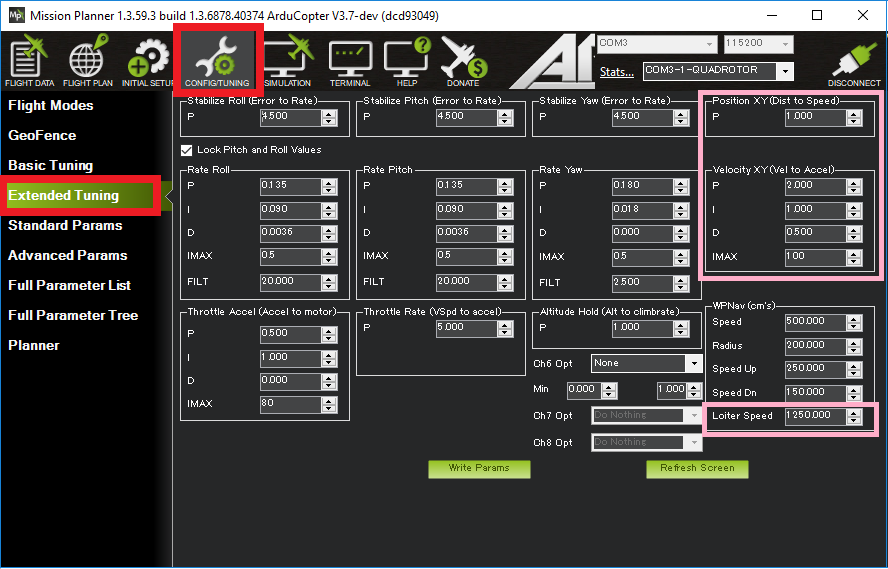
\includegraphics[width=100mm]{MP_Tuning}\\
\end{figure}
\end{onlyenv}
\end{itemize}


\end{frame}

\begin{frame}[t]{Nastavenie parametrov: Ziegler Nichols 1}
\begin{itemize}
  \item<1-> Heuristika\footnote{fuck around, find out} vs.  pseudo-heuristický prístup: Ziegler-Nicholsova (ZN) metóda: \citep{Ziegler1942}
  \item<2-> Nastavme $K_I$, $K_D$ zložky nulové a zvyšujme $K_P$, kým nedostaneme na hranu stability s konzistentnými osciláciami. Tam sme našli $K_{P\max}$ a perióda oscilácii bude $T_{\max}$.
  \item<3-> Opakujeme pre každú slučku, poprípade pre každú os (dá sa aj priviazať dron)
  \item<4-> Na základe týchto hodnôt môžeme z tabuľky na základe pseudoheuristiky vybrať ladenie.

  \begin{onlyenv}<3>
  \begin{figure}
\centering
  \includegraphics[width=40mm]{DroneBench}\\
\end{figure}
\end{onlyenv}

  \begin{onlyenv}<4>
\begin{table}[]
\caption{}
\label{tab:my-table}
\footnotesize
\begin{tabular}{llllll}
 & $K_P$     & $T_I$     & $T_D$      & $K_I$        & $K_D$     \\
\textbf{P }  & 0.5$K_{P\max}$  & -       &  -       &    -       &  -       \\
\textbf{PI } & 0.45$K_{P\max}$ & 0.80$T_{\max}$ &-         & 0.54$K_{P\max}$/$T_{\max}$ &         \\
\textbf{PD}  & 0.8$K_{P\max}$  &  -      & 0.125$T_{\max}$ &  -         & 0.10$K_{P\max}$  \\
\textbf{PID} & 0.6$K_{P\max}$  & 0.5$T_{\max}$  & 0.125$T_{\max}$ & 1.2$K_{P\max}$/$T_{\max}$  & 0.075$K_{P\max}$
\end{tabular}
\end{table}
\end{onlyenv}


\end{itemize}


\end{frame}

\begin{frame}[t]{Nastavenie parametrov: Ziegler Nichols 2}
\begin{itemize}
  \item<1-> \textbf{Výhody:} Jednoduché
  \item<2-> \textbf{Nevýhody:} tlačí to quad na hranu stability, určite nebude ``optimálne'' pre všetky prípady a od 1942 máme lepšie metódy. Nastavené na maximálne odstránenie porúch, náchylné na agresívne riadenie s prestrelom \cite{Bequette2010}
     \item<3-> Môžeme podobné experimentálne dáta získať aj zo skokovej odozvy
  \item<4-> ArduPilot (ArduCopter) --- ``AutoTuning'' Napodobňuje túto heuristiku (ale nie je to ZN) \citep{AP:LogSeminar}
  \begin{itemize}
  \item Zvyšuje P parameter pomaly
  \item Akonáhle deteguje osciláciu, zníži P parameter
  \item Opakuje pre iné zložky/slučky
\end{itemize}
\item<5-> PX4 dlho nemal vstavanú ``autotune'' funkciu \citep{Bolton2018}, momentálne využíva na odhad SISO linearizovaný model 2. rádu  (bez prepojenia medzi osami) \citep{PX4:PIDTuning}
\end{itemize}

\end{frame}


\begin{frame}[t]{Nastavenie parametrov}
\begin{itemize}
  \item<1-> Cohen Coon je založené na ZN, pridá aj oneskorenie sústavy \citep{Joseph2018} (nie je typicky problém pri quadoch)
  \item<2-> Chien, Hrones a Reswickova (CHR) metóda, taktiež založené na ZN. Vyladené na maximalizáciu rýchlosti odozvy bez prestrelu (alebo 20\%) \citep{Hambali2014}.

\end{itemize}
\end{frame} 